\chapter{Simulation of radiative effects}
\label{rad_eff}
%Ref. to Mo and Tsai. with brief overview. Mention s1, s2, and s3. Parameter $\Delta$ choice. How the shifted momenta of the final hadrons are obtained for the case of a photon emission. Interpolation of the integral cross sections for the purpose of rad. eff. calculations. 
%Plots: Missing mass distribution with tail in comparison with data. Distribution of the emitted photon energy.


In order to simulate radiative effects (RE) the Mo and Tsai approach~\cite{Mo:1968cg} was chosen. This approach allows to calculate radiative integral cross sections from the given nonradiative ones in each $(W,~Q^{2})$ point. In~\cite{Mo:1968cg} this is applied to the inclusive case, while here double pion integral cross sections are used instead. 

It is essential that approach~\cite{Mo:1968cg} only accounts for the change of cross section values, therefore an additional procedure (discussed below) is used to generate the energy of the radiative photon and to account for the shift in $W$ and $Q^2$ caused by RE.

It also needs to be mentioned that approach~\cite{Mo:1968cg} assumes that radiative photons are emitted colliniarly to the in- and outgoing electron directions (so-called "peaking approximation"). The minimal energy of the emitted radiative photon is a free parameter. It is denoted as $\Delta$ and chosen to be equal to 10~MeV. In~\cite{Mo:1968cg} it is claimed that the result was found to be insensitive to the choice of $\Delta$ value, however this value must be smaller than the resolution of the experiment.  

% There is a free parameter in this approach it is the minimal energy of the emitted radiative photon $(\Delta)$. The $\Delta$ is chosen to be equal to 10~MeV, but the result was found to be insensitive to the $\Delta$ value choice.  

As it is derived in~\cite{Mo:1968cg} (Eq. (IV.1) on page 213) the radiative cross section in each ($W$,~$Q^2$) point is given by~\footnote[1]{Note that~\cite{Mo:1968cg} assumes the cross section to be differential in ($\Omega$,~$E_{e'}$), while TWOPEG assumes it to be differential in ($W$,~$Q^2$). Therefore, the nonradiative hadronic cross section is taken for the needed ($W$,~$Q^2$) point and then multiplied by the virtual photon flux $\Gamma_{v} = \frac{\alpha}{4\pi^2}\frac{E_{e'}}{E_{beam}m_{p}}\frac{(W^{2}-m_{p}^{2})}{(1-\varepsilon_{T})Q^{2}}$, which is connected with the one defined by~Eq.\eqref{flux} via the Jacobian for the ($W$,~$Q^2$)$\rightarrow$($\Omega$,~$E_{e'}$) coordinate transformation.}

\begin{equation}
\frac{d\sigma_{rad}}{d\Omega  dE_{e'}}(W,Q^{2}) = S_{1} + S_{2} + S_{3}.
\label{eq:rad_tot}
\end{equation}

Three terms in Eq.~\eqref{eq:rad_tot} correspond to various regions of integration in Fig.~3 on page 216 of~\cite{Mo:1968cg}. Contribution from region four in this figure is neglected in order to save computation time.

The term $S_{1}$ corresponds to the so-called "soft radiation", in which the energy of the radiated photon is less than $\Delta$. The two remaining terms correspond to the so-called "hard radiation", in which the energy of the radiated photon is greater than $\Delta$. $S_{2}$ accounts for the changing initial electron energy and $S_{3}$ for the changing scattered electron energy.

Let's look at each term of Eq.~\eqref{eq:rad_tot} in more detail.
\begin{enumerate}

\item $S_{1}$ can be factorized in the following way~\footnote[2]{The Eq.~\eqref{eq:rad_s1} is coded in the function {\em s1\_radsoft} and embedded in {\em radcorr.cxx}.} (see Eq.~(IV.1) in~\cite{Mo:1968cg}).
\begin{equation}
S_{1}(W,Q^2) = \frac{d\sigma_{norad}}{d\Omega  dE_{e'}}(W,Q^2)\cdot R_{soft} = \frac{d\sigma_{norad}}{d\Omega  dE_{e'}}(W,Q^2)\cdot e^{\delta_{t}+\delta_{r}},
\label{eq:rad_s1}
\end{equation} 
where $\delta_{t}$ corresponds to the straggling in the target medium, while $\delta_{r}$ corresponds to the radiative correction to continuum spectrum, both of them are defined on page~214 in~\cite{Mo:1968cg}.

Hence the value of $S_1$ at a given ($W$,$Q^2$) point is determined by the nonradiative cross section taken exactly at this point and multiplied by the factor $R_{soft}$.


\item $S_{2}$ is given by~\footnote[3]{The Eq.~\eqref{eq:rad_s2} is coded in the function {\em s2\_radhardini} and embedded in {\em radcorr.cxx}.}
\begin{equation}
\begin{aligned}
S_{2}(W,Q^2) = \int\limits_{\Delta}^{\omega_{max}^{ini}}\rho_{ini}\frac{d\sigma_{norad}}{d\Omega  dE_{e'}}(\widetilde{W},\widetilde{Q^{2}})d\omega, \\
\omega_{max}^{ini} = E_{beam} - \frac{2m_{\pi}^2 + 2m_{p}m_{\pi} + m_{p}E_{e'}}{m_{p}-E_{e'}(1-cos\theta_{e'})},
\label{eq:rad_s2}
\end{aligned}
\end{equation}

where $\omega_{max}^{ini}$ is the maximal energy of the photon that can be emitted by the initial electron assuming two pion production, $\omega$ is the energy of the radiated photon, $\rho_{ini}$ is the part of the integrand defined by Eq.~(IV.1) in~\cite{Mo:1968cg}. $\widetilde{W}$ and $\widetilde{Q^{2}}$ are the shifted values of $W$ and $Q^{2}$ for the given $\omega$ value. $m_{p}$ and $m_{\pi}$ are the proton and charged pion masses, respectively. $E_{beam}$ is the beam energy defined as an input parameter, $E_{e'}$ and $\theta_{e'}$ are the scattered electron energy and polar angle, respectively, given by Eq.~\eqref{eq:el_in_lab}.

It is essential that $S_2$ is calculated numerically as an integral over the radiated photon energy $\omega$, which varies from $\Delta$ to $\omega_{max}^{ini}$ in increments of $\frac{\omega_{max}^{ini}-\Delta}{800}$. Each $\omega$-point of this grid corresponds to the distinct value of the initial electron energy $E_{beam} - \omega$, which in turn corresponds to the shift of the ($\widetilde{W}, \widetilde{Q^{2}}$) values from their initial values. Thus the value of $S_2$ at the point ($W$, $Q^2$) is calculated as an integral of the integrand that is taken for different shifted ($\widetilde{W}, \widetilde{Q^{2}}$) points on this grid. 


\item $S_{3}$ is given by~\footnote[4]{The Eq.~\eqref{eq:rad_s3} is coded in the function {\em s3\_radhardfin} and embedded in {\em radcorr.cxx}.}
\begin{equation}
\begin{aligned}
S_{3}(W,Q^2) = \int\limits_{\Delta}^{\omega_{max}^{fin}}\rho_{fin}\frac{d\sigma_{norad}}{d\Omega  d\widetilde{E_{e'}}}(\widetilde{W},\widetilde{Q^{2}})d\omega, \\
\omega_{max}^{fin} = \frac{m_{p}E_{beam} - 2m_{p}m_{\pi} - 2m_{\pi}^2}{m_{p} + E_{beam}(1 - cos\theta_{e'})} - E_{e'},
\label{eq:rad_s3}
\end{aligned}
\end{equation}

where $\omega_{max}^{fin}$ is the maximal energy of the photon that can be emitted by the scattered electron assuming two pion production and $\rho_{fin}$  the part of the integrand defined by Eq.~(IV.1) in~\cite{Mo:1968cg}. 

As in the previous case $S_3$ is calculated numerically as an integral over the radiated photon energy $\omega$, which varies from $\Delta$ to $\omega_{max}^{fin}$ in increments of $\frac{\omega_{max}^{fin}-\Delta}{800}$. Each $\omega$-point of this grid corresponds to the distinct value of the scattered electron energy $\widetilde{E_{e'}} = E_{e'} + \omega$, which in turn corresponds to the ($\widetilde{W}, \widetilde{Q^{2}}$) values shifted from the initial ones. Thus the value of $S_3$ at the point ($W$, $Q^2$) is calculated as an integral of the integrand that is taken for different shifted ($\widetilde{W}, \widetilde{Q^{2}}$) points on this grid. 

\end{enumerate}

The nonradiative integral cross sections, which are needed to compute $S_1$, $S_2$, and $S_3$ are an issue of special attention. The subroutine that simulates RE should have access to the nonradiative integral cross sections for each desired point in $W$ and $Q^2$. Although TWOPEG calculates the cross section value as a weight for each event, it is not justified to use these implemented into the EG cross sections for the purpose of RE simulation. The reason for that is the following: these cross sections are five-differential, therefore, in order to be used for the RE simulation they must firstly be obtained on the five-dimensional grid in final hadron variables and then be integrated over that grid. But for each generated event it would happen more than thousand times, that inevitably leads to an incredible increase in the event generation time.

The following alternative can be used instead: the EG should have direct access to the integral cross sections.
For this purpose, the integrated structure functions $\sigma_{T}$ and $\sigma_{L}$ were obtained from TWOPEG itself (see Sect.~\ref{unfold})  
 on the ($W$,~$Q^2$) grid with bin widths 25~MeV in $W$ and 0.05~GeV$^2$ in $Q^2$ in the limits $[1.2625,\;3.0125]$~GeV in $W$ and $[0.0005,\;1.3]$~GeV$^2$ in $Q^2$, respectively. These structure functions were tabulated in the text files that are located in the folder {\em "int\_sec\_new"}. A two-dimensional linear interpolation is used in order to obtain these structure functions in any given ($W$, $Q^2$) point within the limits described above. Then $\sigma_{T}$ and $\sigma_{L}$ are combined into the full cross section for the given beam energy according to Eq.~\eqref{eq:str_fun_decomp}.
For $W > 3.0125$~GeV the cross section is assumed to be the same as at $W = 3.0125$~GeV for each $Q^2$ point, and for $Q^2 > 1.3$~GeV$^2$ the cross section value at $Q^2 = 1.3$~GeV$^2$ for each $W$ point is scaled with the dependency given by~Eq.~\eqref{eq:q2_dep}.  The interpolation time appears to be negligible in comparison with the time needed to produce the cross section on the five-dimensional grid with the subsequent integration. Therefore, using of this approach simulating of RE increases the event generation time only slightly. 

After the values of $S_1$, $S_2$, and $S_3$ are obtained the following factor can be calculated for each event 
\begin{equation}
f_{rc} (W,Q^2) = \left [S_1+S_2+S_3\right ]/\left [\frac{d\sigma}{d\Omega dE_{e'}}(W,Q^2)\right ].
\end{equation}

This factor shows how the radiative cross section is different from the nonradiative one for each given $W$ and $Q^2$ and is applied as an additional weight factor for each event together with the conventional one $f_{cr~sect}$, which carries information about nonradiative cross section and is discussed in Sect.~\ref{sect:data}.

However, the cross section change due to RE is not the only issue we are interested in. One also wants to simulate the radiative tail in distributions like missing masses, which appears due to the mismatch between the hadron and lepton momenta. This mismatch is the consequence of the fact that ($W$,~$Q^2$) values obtained from the initial and scattered electrons, which suffer from RE, are not those for which final hadrons are produced. To simulate this effect one needs to account for the shift in the ($W$,~$Q^2$) values due to RE, which in turn implies the generation of the radiated photon energy.

To generate the radiated photon energy the random number $R$ is generated in the limits [0,~1]. Then three distinct cases are considered.

\begin{itemize}

\item $0 < R < \frac{S_1}{S_1+S_2+S_3}$

This case corresponds to the so-called "soft" scenario, in which the energy of the radiated photon $E_{rad}$ is less than $\Delta$ and considered to be zero, and ($W$,~$Q^2$) values are considered to be unchanged,

\begin{equation}
\begin{aligned}
& E_{rad} = 0,\\
& \widetilde{Q^2} = Q^2,\\
& \widetilde{W} = W.
\label{eq:first_case}
\end{aligned}
\end{equation}

\item $\frac{S_1}{S_1+S_2+S_3} < R < \frac{S_1+S_2}{S_1+S_2+S_3}$

This case corresponds to the emission of a "hard" photon by the initial electron. The photon energy $E_{rad}$ is generated in the limits [$\Delta$,~$\omega_{max}^{ini}$] according to the probability density~\footnote[5]{Using ROOT it is convenient to do it in the following way.\\
TH1F *h\_radhardini = new TH1F("h\_radhardini","h\_radhardini",800,$\Delta$,$\omega_{max}^{ini}$);\\
for (Int\_t i=0;i$<$800;i++) h\_radhardini$\rightarrow$SetBinContent(i+1,(ARR[i]+ARR[i+1])/2.);\\
R2[0] = hardini\_rndm.Uniform(0.,1.);\\
h\_radhardini$\rightarrow$GetQuantiles(1,eran,R2);\\where ARR[i] is the value of the integrand in Eq.~\eqref{eq:rad_s2} taken on the $\omega$-grid and eran[0] is the photon energy denoted as $E_{rad}$ in the text. } given by the integrand in Eq.~\eqref{eq:rad_s2}. In this case

\begin{equation}
\begin{aligned}
& \widetilde{E}_{beam} = E_{beam} - E_{rad},\\
& \widetilde{Q^2} = 2\widetilde{E}_{beam}E_{e'}(1 - cos\theta_{e'}),\\
& \widetilde{W} = \sqrt{m_{p}^{2} - \widetilde{Q^2} + 2(\widetilde{E}_{beam} - E_{e'})m_{p}},
\label{eq:2nd_case}
\end{aligned}
\end{equation}

where $E_{e'}$ and $\theta_{e'}$ are assumed to be unchanged.

\item $\frac{S_1+S_2}{S_1+S_2+S_3} < R < 1$

This case corresponds to the emission of a "hard" photon by the final electron. The photon energy $E_{rad}$ is generated in the limits [$\Delta$,~$\omega_{max}^{fin}$] according to the probability density given by the integrand in Eq.~\eqref{eq:rad_s3}. In this case

\begin{equation}
\begin{aligned}
& \widetilde{E}_{e'} = E_{e'} + E_{rad},\\
& \widetilde{Q^2} = 2E_{beam}\widetilde{E}_{e'}(1 - cos\theta_{e'}),\\
& \widetilde{W} = \sqrt{m_{p}^{2} - \widetilde{Q^2} + 2(E_{beam} - \widetilde{E}_{e'})m_{p}},
\label{eq:3rd_case}
\end{aligned}
\end{equation}

where $E_{beam}$ and $\theta_{e'}$ are assumed to be unchanged.

\end{itemize}


Now these shifted ($\widetilde{W}$,~$\widetilde{Q^2}$) values are sent as an input to the subroutine that calculates the four-momenta of the final hadrons in the lab frame (see Sect.~\ref{sect:cms_to_lab_trans}). As a result the calculated hadron momenta account for the shift of the ($W$,~$Q^2$) values due to RE. However, the final electron is assumed to be unchanged and still to be defined by Eq.~\eqref{eq:el_in_lab} for the originally generated ($W$,~$Q^2$) values, as well as the initial electron that is assumed to have the unchanged beam energy $E_{beam}$. This corresponds to the real experiment, where one loses information about the change of the lepton momenta due to RE, and the radiative tail in distributions like missing masses appears.

\begin{figure}[!ht]
\begin{center}
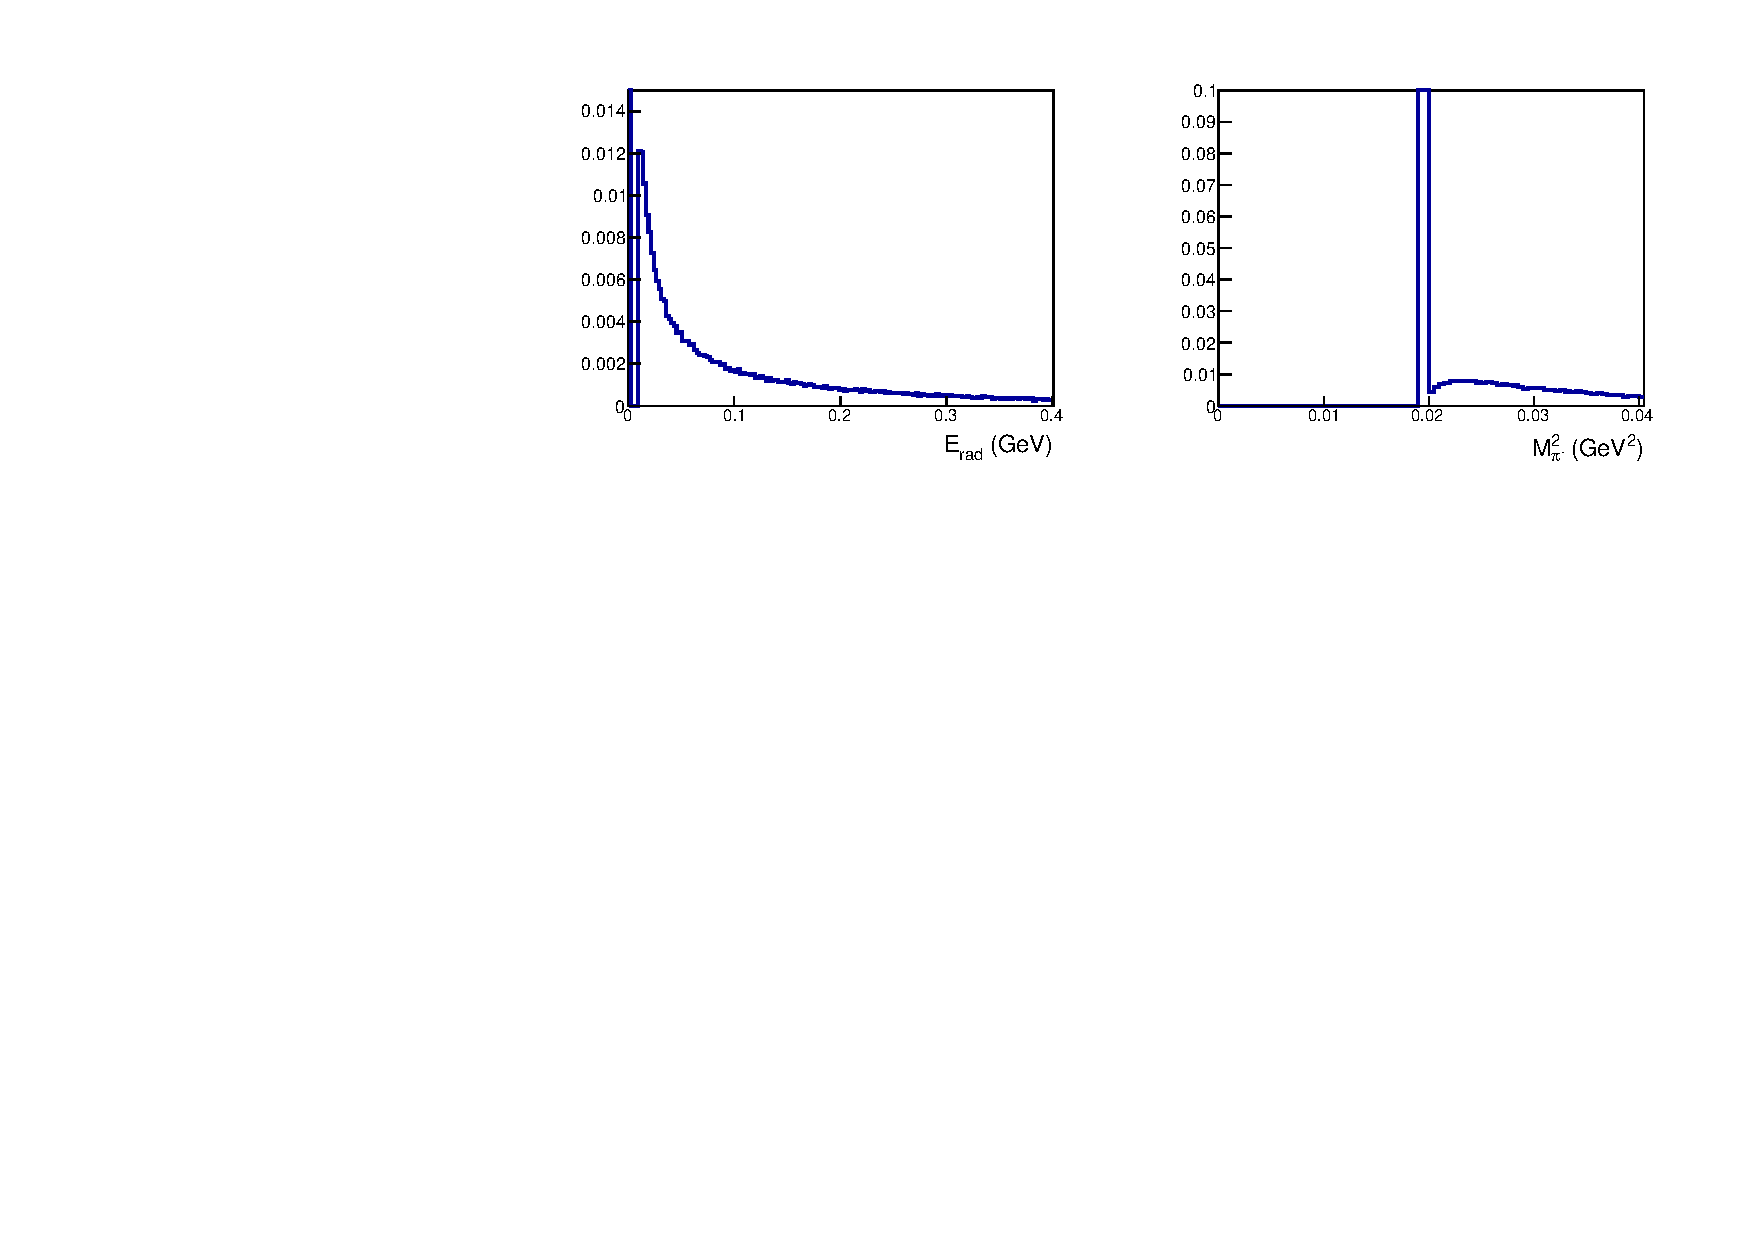
\includegraphics[height=0.4\textwidth]{pictures/radeff/miss_mass_pim_eradgam.pdf}
\end{center}
\vspace{-0.6cm}
\caption{\small Left plot: the distribution of the radiated photon energy $E_{rad}$. Right plot: the distribution of missing mass squared of $\pi^{-}$, which is calculated according to Eq.~\eqref{eq:miss_mass_pim}. Both histograms are normalized in a way that the maxima of the main peaks at zero (left) and at pion mass squared (right) are equal to one. The example is given for the case of $E_{beam} = 2$~GeV, $1.6 < W < 1.8$~GeV, and $0.4 < Q^{2} < 0.5$~GeV$^{2}$.}
\label{fig:miss_mass_pim_eradgam}
\end{figure}

Figure~\ref{fig:miss_mass_pim_eradgam} shows the distributions of the radiated photon energy (left plot) and missing mass squared of the $\pi^{-}$ (right plot). The latter is calculated by
\begin{equation} \label{eq:miss_mass_pim}
M_{\pi^{-}}^{2} = (P_{p} + P_{e} - P_{e'} - \widetilde{P}_{p'} - \widetilde{P}_{\pi^{+}})^{2},
\end{equation}

where $P_{i}$ is the four-momentum of the particle $i$. $\widetilde{P}_{p'}$ and $\widetilde{P}_{\pi^{+}}$ correspond to the hadron momenta calculated for the shifted ($\widetilde{W}$,~$\widetilde{Q^2}$) values, while $P_{e}$ and $P_{e'}$ correspond to the initial unshifted ($W$,~$Q^2$) values. This mimics the conditions of real experiment and leads to the radiative tail, which is clearly seen in the right plot of Fig.~\ref{fig:miss_mass_pim_eradgam}.






